% Rework the sentence  JOM
\textbf{
The GAs were applied to the selection of features for the
prediction of effective temperature from both, noiseless and noisy spectra.
For the IRTF wavelength range and resolution, results in the features have been included
in Table~\ref{tab:irtf-teff-noisy}. 
}
% End of update
Features are ordered by the
fitness value (according to the AIC criterion, as explained in Eq.~\ref{eq:AIC}) and 
we only consider features that are present in at least 5 sets.

% When noise is added to the BT-Settl spectra, we obtain the features
% included in Table \ref{tab:irtf-teff-noisy}.

Table % \ref{tab:irtf-teff-noiseless} and 
\ref{tab:irtf-teff-noisy}
show a very wide variety of features with very few repetitions. Only
spectral features 4, 5, 6, and 9 in the SNR=50 experiment are found
too in the SNR=$\infty$ and SNR=10 feature sets (albeit with different
continuum definitions). This reinforces the impression that the
information useful for the estimation of the effective temperatures is
spread over the entire IRTF spectrum.
% Removing Table A3 => JOM
\textbf{
As a reference, it is used the Table~3 defined in \cite{cesetti}, which
%~\ref{tab:irtf-cesetti} 
lists the features found using sensitivity maps.
}
% End of changes


\begin{figure}
 \captionsetup[subfloat]{farskip=2pt,captionskip=-18pt}
 \vspace*{-10pt}
 \subfloat[BT\_Settl noiseless spectra \label{fig:irtf-teff-inf}] {    
    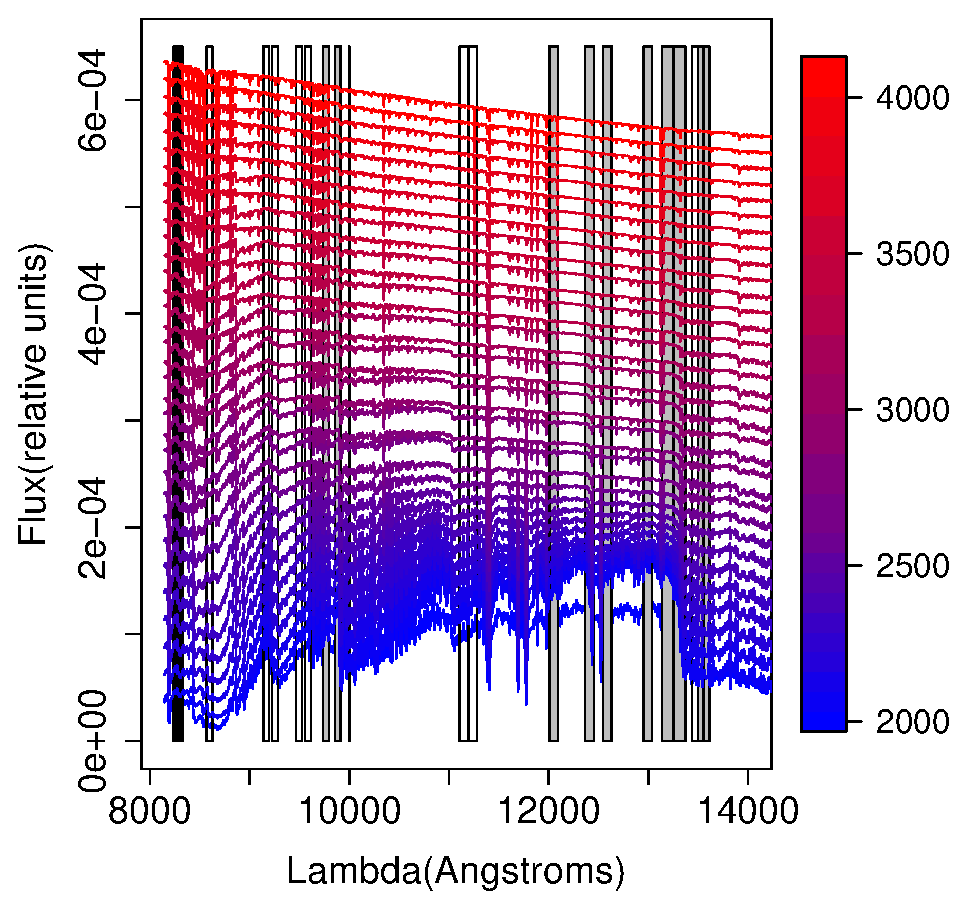
\includegraphics[width=0.45\textwidth]{figs/BT-spectraAtIRTF-Inf-teff}}\\[-9ex]

 \subfloat[BT\_Settl spectra of SNR=10 \label{fig:irtf-teff-10}] { 
    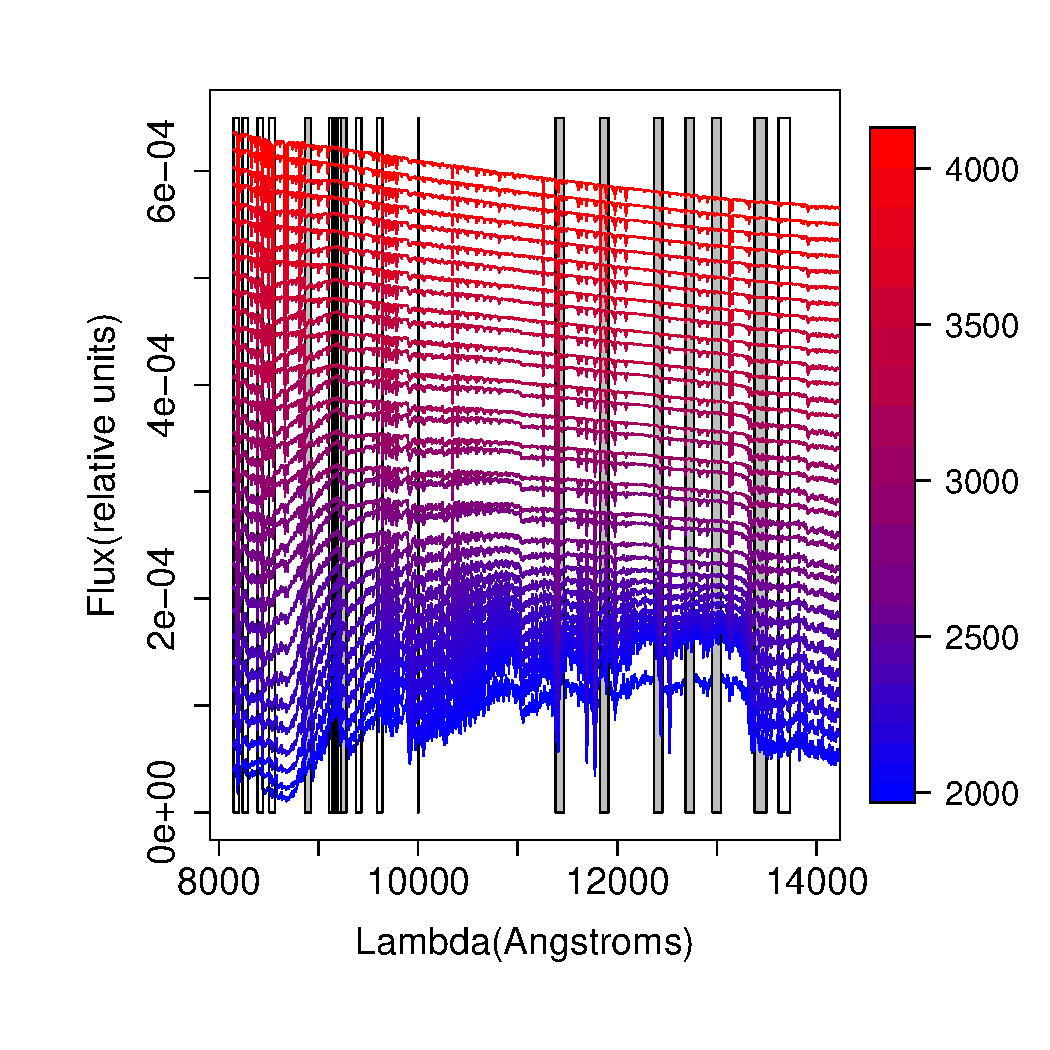
\includegraphics[width=0.45\textwidth]{figs/BT-spectraAtIRTF-10-teff}}\\[-9ex]

 \subfloat[BT\_Settl spectra of SNR=50 \label{fig:irtf-teff-50}] {  
    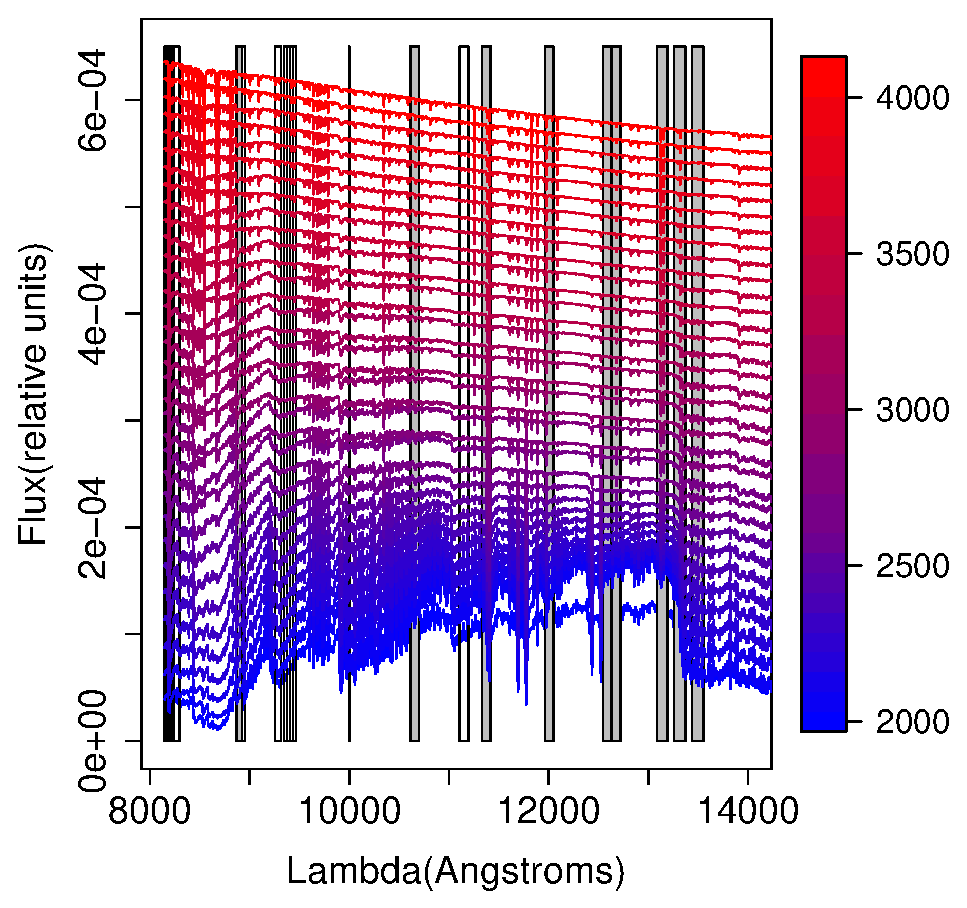
\includegraphics[width=0.45\textwidth]{figs/BT-spectraAtIRTF-50-teff}}\\[-7ex]
%
 \caption{Features selected by the GA for predicting $T_{eff}$ using
    BT\_Settl synthetic spectra in the IRTF wavelength range
    and resolution. The BT\ Settl spectra are plot in a colour scale
    that ranges from blue (2000 K) to red (4100 K). The empty boxes
    correspond to the selected features and the grey boxes to the
    continuum bands.}
 \label{fig:IRTF-teff} 
\end{figure}

%

\begin{figure}
 \captionsetup[subfloat]{farskip=2pt,captionskip=-18pt}
 \vspace*{-10pt}
 \subfloat[BT\_Settl noiseless spectra \label{fig:irtf-logg-inf}] {  
    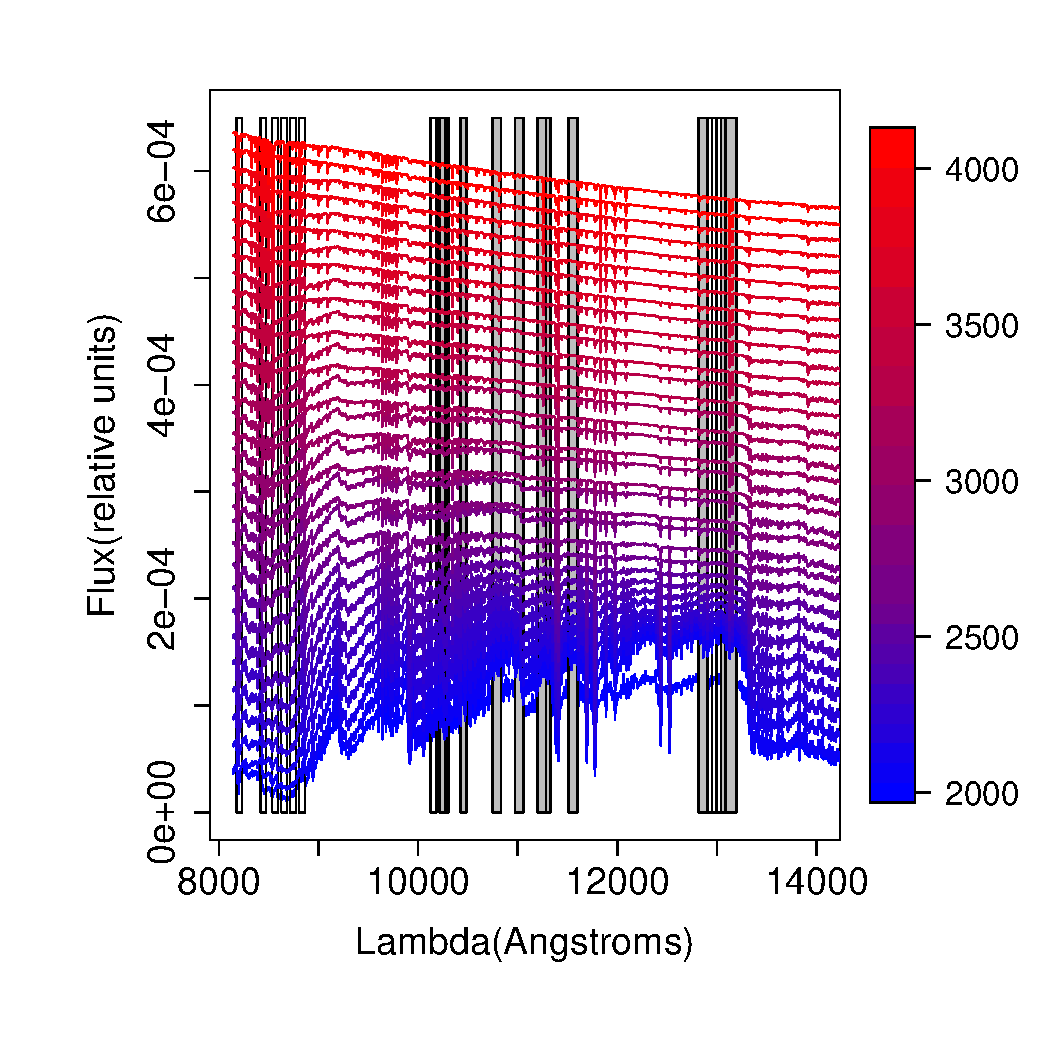
\includegraphics[width=0.45\textwidth]{figs/BT-spectraAtIRTF-Inf-logg}}\\[-9ex]

 \subfloat[BT\_Settl spectra of SNR=10 \label{fig:irtf-logg-10}] { 
    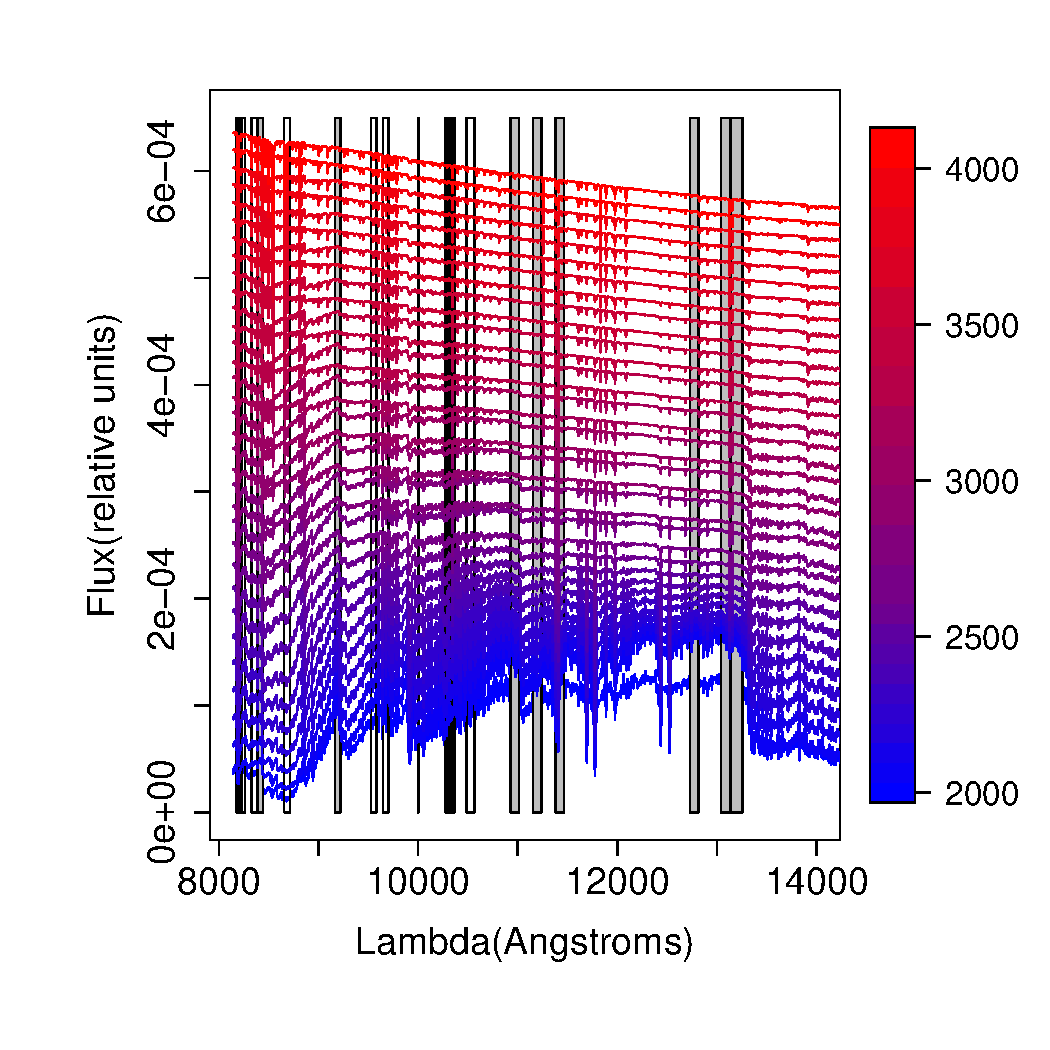
\includegraphics[width=0.45\textwidth]{figs/BT-spectraAtIRTF-10-logg}}\\[-9ex]

 \subfloat[BT\_Settl spectra of SNR=50 \label{fig:irtf-logg-10}] { 
    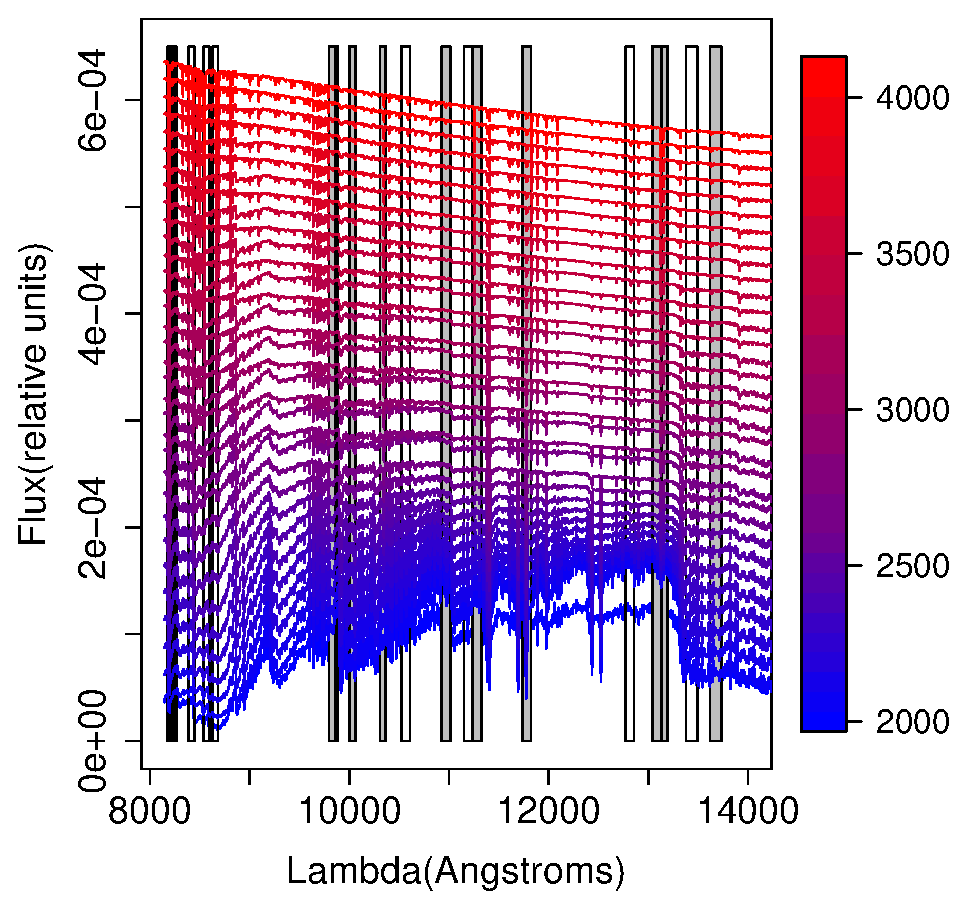
\includegraphics[width=0.45\textwidth]{figs/BT-spectraAtIRTF-50-logg}}\\[-7ex]

 \caption{Features selected by the GA for predicting $\log(g)$ using
    BT\_Settl synthetic spectra in the IRTF wavelength range
    and resolution. The BT\ Settl spectra are plot in a colour scale
    that ranges from blue (2000 K) to red (4100 K). The empty boxes
    correspond to the selected features and the grey boxes to the
    continuum bands.}
 \label{fig:IRTF-logg} 
\end {figure}

% %
% 
\begin{figure}
 \captionsetup[subfloat]{farskip=2pt,captionskip=-18pt}
 \vspace*{-10pt}
 \subfloat[BT\_Settl noiseless spectra \label{fig:irtf-met-inf}] { 
    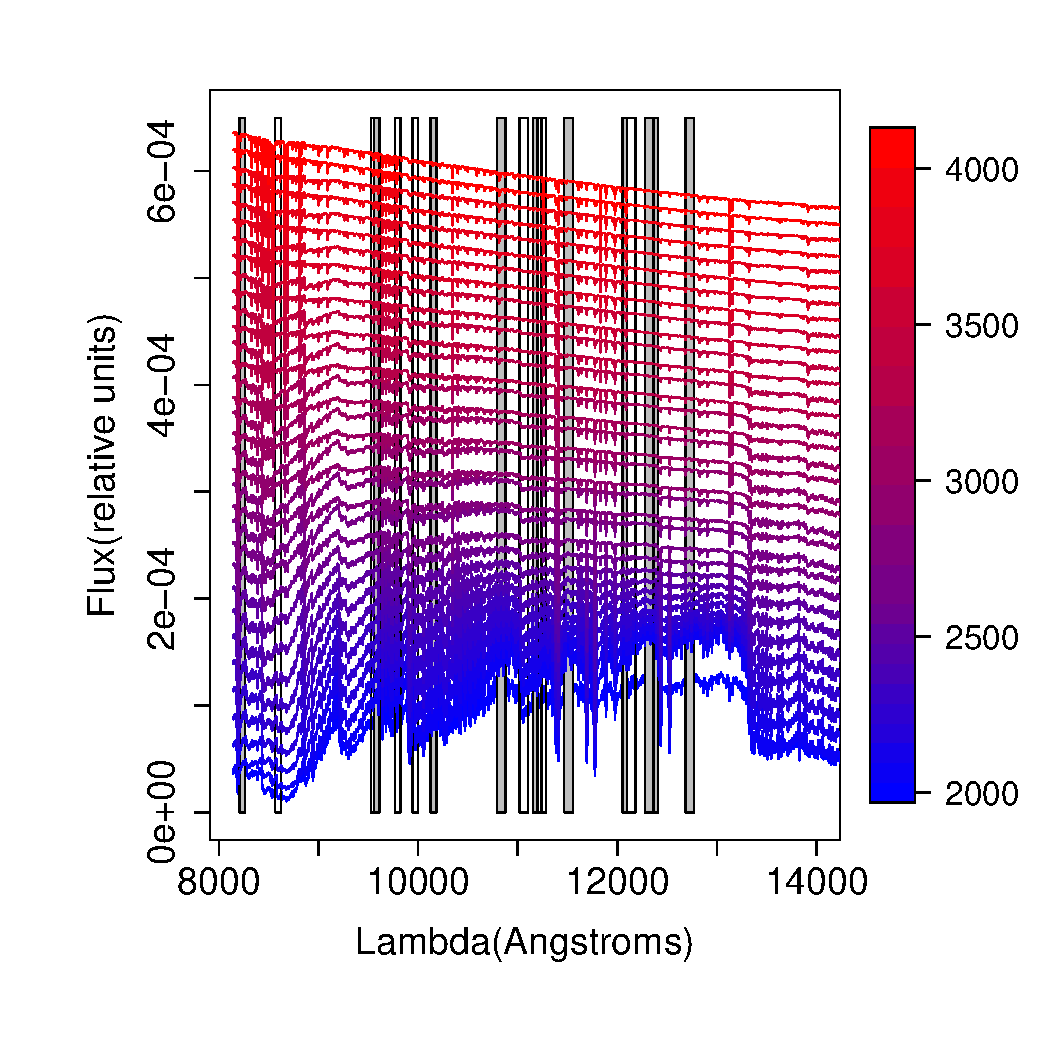
\includegraphics[width=0.45\textwidth]{figs/BT-spectraAtIRTF-Inf-mh}}\\[-9ex]

 \subfloat[BT\_Settl spectra of SNR=10 \label{fig:irtf-met-10}] { 
    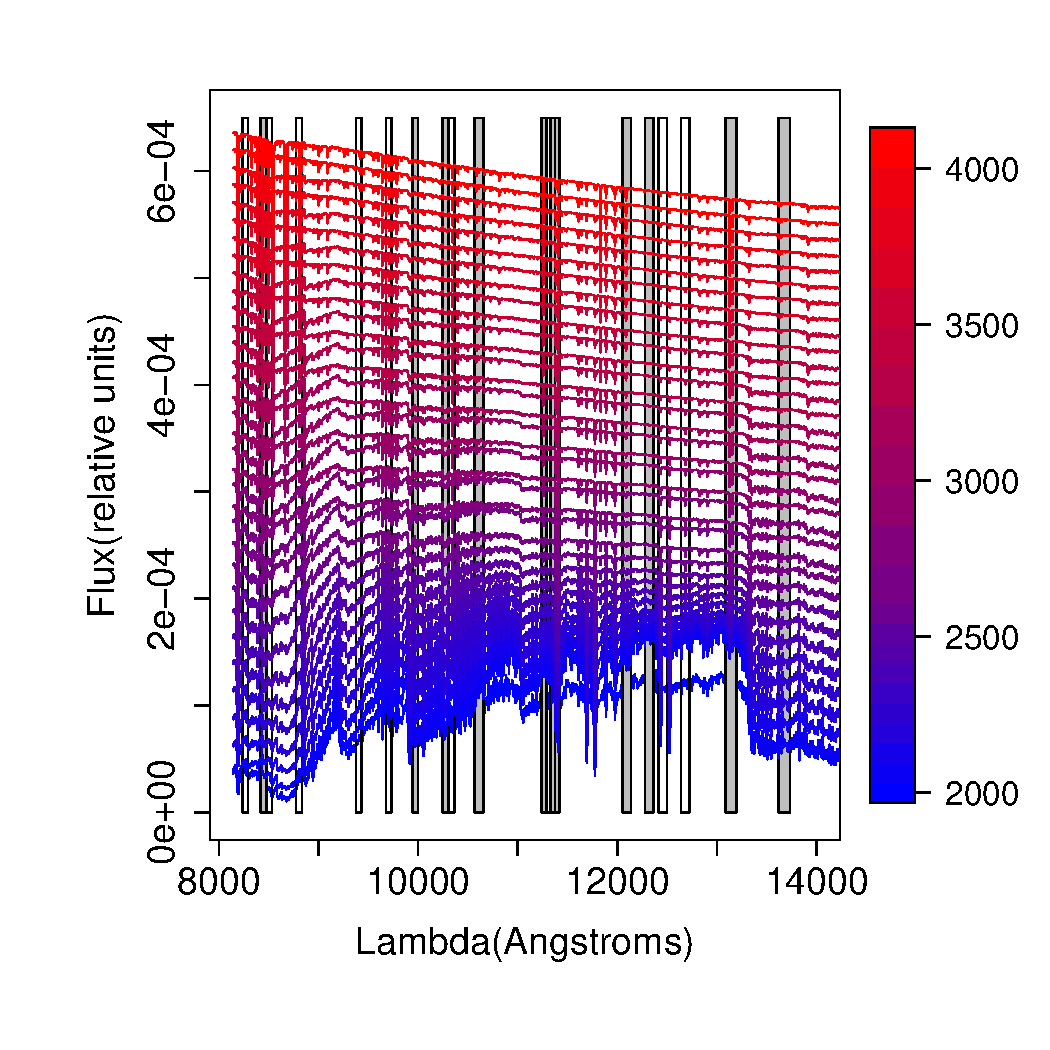
\includegraphics[width=0.45\textwidth]{figs/BT-spectraAtIRTF-10-mh}}\\[-9ex]

 \subfloat[BT\_Settl spectra of SNR=50 \label{fig:irtf-met-50}] { 
    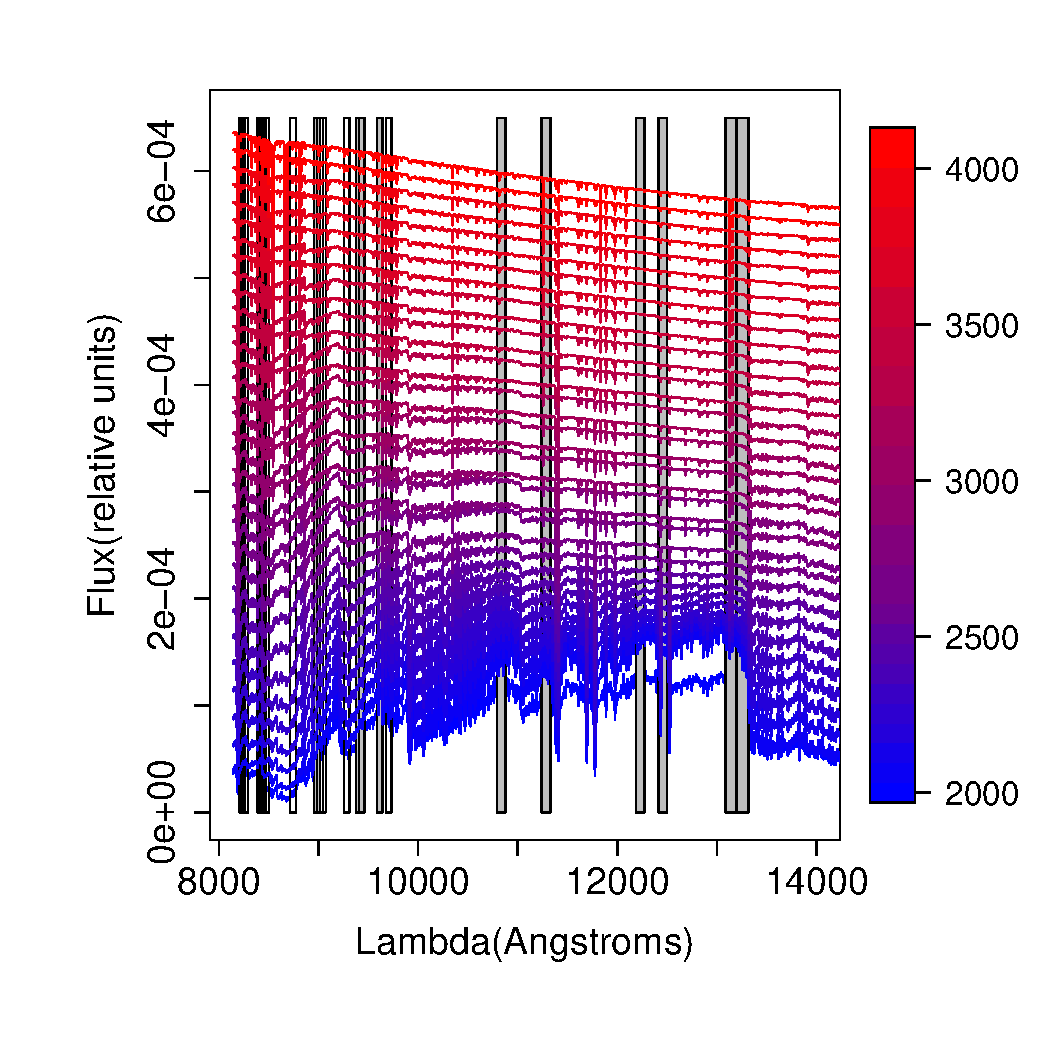
\includegraphics[width=0.45\textwidth]{figs/BT-spectraAtIRTF-50-mh}}\\[-7ex]

 \caption{Features selected by the GA for predicting [M/H] using
    BT\_Settl synthetic spectra in the IRTF wavelength range
    and resolution. The BT\ Settl spectra are plot in a colour scale
    that ranges from blue (2000 K) to red (4100 K). The empty boxes
    correspond to the selected features and the grey boxes to the
    continuum bands.}
 \label{fig:IRTF-met}
\end {figure}



For gravity estimation (on a logarithmic scale), the GA search
procedure produces the features presented in
Table % \ref{tab:irtf-logg-noiseless} and 
\ref{tab:irtf-logg-noisy} for
the noiseless signal and signal-to-noise ratios of 10 and 50,
respectively. In a similar way, the best features found 
by the GA for metallicity estimation are listed in % Table~\ref{tab:irtf-met-noiseless} for the noiseless BT-Settl
% spectra, and in 
Table~\ref{tab:irtf-met-noisy} for signal-to-noise
ratios equal to $ \infty, 10 $ and $ 50 $.

Figures \ref{fig:IRTF-teff}-\ref{fig:IRTF-met} show
graphically the band limits listed in
Tables~\ref{tab:irtf-teff-noisy} to \ref{tab:irtf-met-noisy}
% --\ref{tab:irtf-met-noiseless} 
on a collection of spectra from the BT-Settl library.

